\section{Modellierung}

\begin{defi}{Modellierung}
    \emph{Modellierung} übersetzt ein reales Problem (Szenario/Mini-Welt, z.B. die lesenswerten Artikel) in eine \enquote{bearbeitbare} Version, das Modell, um final ein Ergebnis (Datenbankentwurf) systematisch zu entwickeln.

    Ein Modell sollte
    \begin{itemize}
        \item vollständig,
        \item korrekt,
        \item minimal,
        \item verständlich und
        \item erweiterbar
    \end{itemize}
    sein.
\end{defi}

\begin{defi}{ANSI/SPARC-Architektur}
    Die \emph{ANSI-SPARC-Architektur} (auch Drei-Schema-Architektur, Drei-Ebenen-Architektur oder Drei-Ebenen-Schema-Architektur) beschreibt die grundlegende Trennung verschiedener Beschreibungsebenen für Datenbankschemata.

    Die drei Ebenen sind:
    \begin{itemize}
        \item Die \emph{externe Ebene}, die den Benutzern und Anwendungen individuelle Benutzersichten bereitstellt. Beispiele: Formulare, Masken-Layouts, Listen, Schnittstellen.
        \item Die \emph{konzeptionelle Ebene}, in der beschrieben wird, welche Daten in der Datenbank gespeichert sind, sowie deren Beziehungen zueinander. Designziel ist hier eine vollständige und redundanzfreie Darstellung aller zu speichernden Informationen.
              Hier findet die Normalisierung des relationalen Datenbankschemas statt.
        \item Die \emph{interne Ebene} (auch physische Ebene), die die physische Sicht der Datenbank im Computer darstellt.
              In ihr wird beschrieben, wie und wo die Daten in der Datenbank gespeichert werden.
              Designziel ist hier ein effizienter Zugriff auf die gespeicherten Informationen.
              Das wird meistens nur durch eine bewusst in Kauf genommene Redundanz erreicht (z. B. im Index werden die gleichen Daten gespeichert, die auch schon in der Tabelle gespeichert sind).
    \end{itemize}

    Die Vorteile des Drei-Ebenen-Modells sind:
    \begin{itemize}
        \item Physische Datenunabhängigkeit: Die interne Ebene ist von der konzeptionellen und externen Ebene getrennt. Physische Änderungen, z. B. des Speichermediums oder des Datenbankprodukts, wirken sich nicht auf die konzeptionelle oder externe Ebene aus.
        \item Logische Datenunabhängigkeit: Die konzeptionelle und die externe Ebene sind getrennt.
              Dies bedeutet, dass Änderungen an der Datenbankstruktur (konzeptionelle Ebene) keine Auswirkungen auf die externe Ebene, also die Masken-Layouts, Listen und Schnittstellen haben.
    \end{itemize}
\end{defi}

\begin{defi}{Entity-Relationship-Modell}
    Das \emph{Entity-Relationship-Modell} (kurz \emph{ER-Modell}) dient dazu, im Rahmen der semantischen Datenmodellierung den in einem gegebenen Kontext (z. B. einem Projekt zur Erstellung eines Informationssystems) relevanten Ausschnitt der realen Welt zu bestimmen und darzustellen.

    Grundlage der Entity-Relationship-Modelle ist die Typisierung von Objekten, ihrer Beziehungen untereinander und der über sie zu führenden Informationen („Attribute“).
\end{defi}

\begin{defi}{Entität}
    Eine \emph{Entität (\enquote{Entity})} $e$ beschreibt ein individuell identifizierbares Objekt der Wirklichkeit.
    Sie ist damit vergleichbar mit einer Objektinstanz und entspricht einem einzelnen Datensatz in einer Datenbank, z.B. das Pokémon \emph{Glumanda} oder die Attacke \emph{Flammenwurf}.
\end{defi}

\begin{defi}{Entitätstyp}
    Ein \emph{Entitätstyp (\enquote{Entity-Set})} beschreibt eine Menge $E$ von Entitäten $e \in E$ mit gleichen Eigenschaften (Klassifikation), z.B. \enquote{Pokémon}.
    Hier liegt eine Betrachtung als Menge von Objekten zugrunde.

    Ein Entitätstyp ist vergleichbar mit einer Klassenbeschreibung und entspricht damit häufig einer Tabelle in einer relationalen Datenbank, hierbei sind die Spalten die Attribute.
\end{defi}

\begin{defi}{Attribut}
    Eine \emph{Attribut (\enquote{Attribute})} definiert, was über eine Entität (im Kontext) von Interesse ist.
    Eine Entität $e$ ist durch die Werte ihrer Attribute charakterisiert und ein Entitätstyp $E$ durch die Attribute selber.

    Jedem Attribut $A$ ist ein Datentyp $T$ und damit implizit oder auch explizit ein Wertebereich $D$ (\enquote{Domain}) zugeordnet, der festlegt, welche Attributwerte zulässig sind \footnote{Wir schreiben: $A \in D$ oder $A:D$ bzw. $A:T$.} , z.B. \emph{Größe} und \emph{Gewicht} des Pokémon Glumanda vom Typ \texttt{float}, die \emph{Stärke} und \emph{Genauigkeit} der Attacke Flammenwurf vom Typ \texttt{int}.

    Besonders ist der Nullwert \texttt{NULL}.
    Das ist ein spezieller Attributwert, dessen Bedeutung variiert, d.h. z.B. ist der Wert unbekannt oder noch nicht festgelegt oder nicht möglich.
    \texttt{NULL} kann, muss aber nicht, im Wertebereich liegen.

    Wir notieren $E[A_1 : D_1, A_2 : D_2, \ldots, A_n : D_n]$ für einen Entitätstyp $E$ mit den Eigenschaften $A_1, \ldots, A_n$.
    Wertebereiche bzw. Typen werden, wenn nicht relevant, auch ausgelassen.

    $W(D)$ bezeichnet alle real existierenden Werte der Domain $D$ in einer Datenbank.
\end{defi}

\begin{defi}{Zusammengesetztes Attribut}
    \emph{Zusammengesetzte Attribute} haben selbst Attribute, z.B.
    \begin{center}
        \texttt{NAME: [Vorname: char(30), Nachname: char(30)]}

        \texttt{ANSCHRIFT: [Straße: char(30), Ort: char(30), PLZ: char(5)]}
    \end{center}

    Die Domain für ein zusammengesetztes Attribut $A$ mit Unterattributen $A_1, \ldots, A_n$ ist dann gegeben mit:
    \[
        A: [A_1 : D_2, \ldots, A_n:D_n]: D_1 \times \ldots \times D_n
    \]
\end{defi}

\begin{defi}{Mehrwertiges Attribut}
    Ein \emph{mehrwertiges Attribut} kann mehrere Ausprägungen  (Werte) haben, z.B.
    \begin{center}
        \texttt{AUTOFARBE: \{char(20)\}}

        \texttt{TELEFONNR: \{char(30)\}}
    \end{center}

    Die Domain für ein mehrwertiges Attribut ist dann gegeben mit
    \[
        E : \{A\}
    \]
\end{defi}

\begin{defi}{Schlüsselkandidat}
    Ein \emph{Schlüsselkandidat}, oder kurz Schlüssel (\enquote{key}), ist ein einwertiges Attribut oder eine Attributkombination, die jede Entität eindeutig identi!ziert.

    Es ist möglich, dass mehrere Schlüsselkandidaten existieren.

    Der sogenannte \emph{Primärschlüssel} ist ein ausgewählter Schlüsselkandidat.
    Seine Primärschlüssel-attribute werden im ER-Diagramm durch Unterstreichung gekennzeichnet.

    Formal wird ein Primärschlüssel wie folgt dargestellt:
    \begin{center}
        \texttt{E: <[Attribute], \{Primärschlüssel\}>}
    \end{center}
    z.B.:
    \begin{center}
        \texttt{Buch: <[InvNr, Titel, Verlag, \{Autor: [Vorname, Nachname]\}], \{InvNr\}>}
    \end{center}
\end{defi}

\begin{defi}{Beziehung}
    Eine \emph{Beziehung (\enquote{Relationship})} erzeugt eine Verknüpfung bzw. einen Zusammenhang zwischen zwei oder mehreren Entitäten.

    Eine Relationship-Menge $R$ entspricht einer mathematischer Relation zwischen $n$ Entity-Mengen $E_i$:
    \[
        R \subseteq E_1 \times \ldots E_n \qquad (\text{häufig} \ n \in \{2, 3\})
    \]
    Eine Relation gibt an, ob eine Entität $e_1 \in E_1$ zu einer anderen Entität $e_2 \in E_2$ in Beziehung steht oder nicht, d.h.
    \[
        (e_1, e_2) \in \R \quad \text{bzw.} \quad (e_1, e_2) \notin \R
    \]

    z.B. gilt also:
    \[
        \text{Pokémon Pikachu \emph{lernt} die Attacke Donner} \ \iff \ (\text{Pikachu}, \text{Donner}) \in \text{lernt}
    \]
\end{defi}

\begin{defi}{Kardinalität}
    Die \emph{Kardinalität} gibt an, zu wie vielen Elementen ein Element in Beziehung steht.

    Es gibt grundsätzlich folgende Abbildungsbeziehungen zwischen Entity-Mengen in der Chen-Notation:
    \begin{itemize}
        \item \emph{1:1} (One-to-One)
        \item \emph{n:1} (Many-to-One)
        \item \emph{1:n} (One-to-Many)
        \item \emph{n:m} (Many-to-Many)
    \end{itemize}

    Die Kardinalität ergibt sich im Wesentlichen aus den Anforderungen und bestimmt ganz maßgeblich den Datenbankentwurf.
\end{defi}

\begin{defi}{Chen-Notation}
    Die \emph{Chen-Notation} ist eine grafische Notation für Entity-Relationship-Modelle.

    Angegeben in der grafischen Darstellung werden die:
    \begin{itemize}
        \item Entitätstypen bzw. Klassen
        \item Kardinalitäten
        \item Beziehungstypen
    \end{itemize}
\end{defi}

\begin{example}{1:1 Relation (Chen-Notation)}
    In Pokémon verleiht im Laufe des Spiels jede \emph{Arena} genau einen \emph{Orden}.

    Damit gilt:
    \begin{center}
        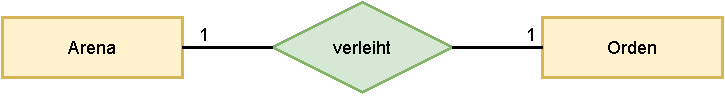
\includegraphics[width=0.7\linewidth]{includes/figures/example_entity_relationship_modell_chen_one_to_one.pdf}
    \end{center}
\end{example}

\begin{example}{1:n Relation (Chen-Notation)}
    In Pokémon hat jede \emph{Arena} mindestens einen, manchmal aber auch mehrere \emph{Arenaleiter}.

    Damit gilt:
    \begin{center}
        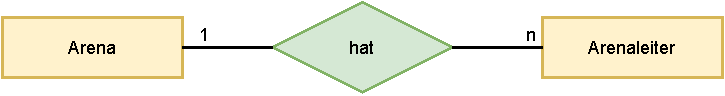
\includegraphics[width=0.7\linewidth]{includes/figures/example_entity_relationship_modell_chen_one_to_many.pdf}
    \end{center}
\end{example}

\begin{example}{n:1 Relation (Chen-Notation)}
    In Pokémon ist jede \emph{Attacke} von genau einem \emph{Typ}.
    Natürlich können aber mehrere \emph{Attacken} auch vom gleichen \emph{Typ} sein.

    Damit gilt:
    \begin{center}
        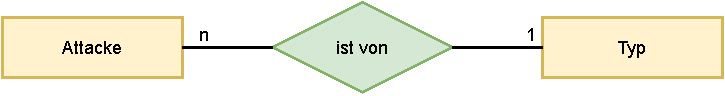
\includegraphics[width=0.7\linewidth]{includes/figures/example_entity_relationship_modell_chen_many_to_one.pdf}
    \end{center}
\end{example}

\begin{example}{n:m Relation (Chen-Notation)}
    In Pokémon kann jedes \emph{Pokémon} einige \emph{Attacken} lernen.
    Die gleiche \emph{Attacke} kann aber gleichzeitig von mehreren \emph{Pokémon} erlernt werden.

    Damit gilt:
    \begin{center}
        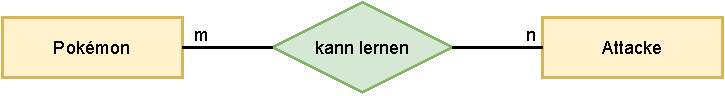
\includegraphics[width=0.7\linewidth]{includes/figures/example_entity_relationship_modell_chen_many_to_many.pdf}
    \end{center}
\end{example}

\begin{example}{Entity-Relationship-Modell}

\end{example}

\begin{example}{}

\end{example}